\documentclass[12pt,a4paper]{article}
\usepackage[utf8]{inputenc}
\usepackage[english]{babel}
\usepackage{amsmath}
\usepackage{amsfonts}
\usepackage{amssymb}
\usepackage{graphicx}
\usepackage{tikz}
\usepackage{algorithm}
\usepackage{algorithmic}
\usepackage{listings}
\usepackage{xcolor}
\definecolor{lightblue}{RGB}{173,216,230}
\definecolor{gold}{RGB}{255,215,0}
\usepackage{geometry}
\usepackage{fancyhdr}
\usepackage{hyperref}
\usepackage{array}
\usepackage{booktabs}
\usepackage{multirow}

\geometry{margin=1in}
\pagestyle{fancy}
\fancyhf{}
\rhead{Dynamic Programming: 0-1 Knapsack}
\lhead{Algorithm Analysis}
\cfoot{\thepage}

% Code listing style
\lstset{
    language=Java,
    basicstyle=\ttfamily\small,
    keywordstyle=\color{blue},
    commentstyle=\color{green},
    stringstyle=\color{red},
    numbers=left,
    numberstyle=\tiny,
    frame=single,
    breaklines=true,
    showstringspaces=false
}

\title{\textbf{Dynamic Programming Analysis: \\The 0-1 Knapsack Problem}}
\author{Algorithm Implementation and Analysis}
\date{\today}

\begin{document}

\maketitle

\tableofcontents
\newpage

\section{Problem Statement}

\subsection{Definition}
The \textbf{0-1 Knapsack Problem} is a classic optimization problem that asks:

\begin{quote}
\textit{Given a knapsack with a fixed weight capacity and a collection of items, each with a specific weight and value, determine the most valuable combination of items that can fit in the knapsack. Each item can be either included (1) or excluded (0), hence the name "0-1" knapsack.}
\end{quote}

\subsection{Real-World Analogy}
Imagine you're going on a hiking trip with a backpack that can carry only 50 pounds. You have various items to choose from:
\begin{itemize}
\item Tent: 10 lbs, Value: \$60 (essential shelter)
\item Sleeping bag: 20 lbs, Value: \$100 (comfort and warmth)
\item Food supplies: 30 lbs, Value: \$120 (nutrition for the trip)
\end{itemize}

You need to maximize the total value while staying within the weight limit. This is exactly what the 0-1 Knapsack problem solves!

\subsection{Mathematical Formulation}
Let:
\begin{itemize}
\item $n$ = number of items
\item $W$ = knapsack capacity
\item $w_i$ = weight of item $i$
\item $v_i$ = value of item $i$
\item $x_i \in \{0, 1\}$ = decision variable (0 = exclude, 1 = include)
\end{itemize}

\textbf{Objective:} Maximize $\sum_{i=1}^{n} v_i \cdot x_i$

\textbf{Subject to:} $\sum_{i=1}^{n} w_i \cdot x_i \leq W$

\section{Problem Visualization}

\subsection{Example Setup}
Let's use our hiking example:
\begin{center}
\begin{tabular}{|c|c|c|c|}
\hline
\textbf{Item} & \textbf{Weight (lbs)} & \textbf{Value (\$)} & \textbf{Value/Weight} \\
\hline
Tent & 10 & 60 & 6.0 \\
Sleeping Bag & 20 & 100 & 5.0 \\
Food Supplies & 30 & 120 & 4.0 \\
\hline
\end{tabular}
\end{center}

\textbf{Capacity:} 50 lbs

\subsection{Decision Tree Visualization}

The decision tree for our 0-1 Knapsack problem can be represented as follows:

\begin{figure}[h]
\centering
\begin{verbatim}
                          Start (0 items, 50 lbs capacity, $0)
                         /                                    \
                      /                                          \
                 No Tent                                      + Tent
          (0 items, 50 lbs, $0)                      (1 item, 40 lbs, $60)
              /            \                              /                \
           /                 \                         /                    \
        No SB               + SB                   No SB                  + SB
   (0, 50, $0)         (1, 30, $100)         (1, 40, $60)         (2, 20, $160)
     /      \             /        \             /        \           /          \
    /        \           /          \           /          \         /            \
 No Food   +Food     No Food     +Food      No Food     +Food    No Food       +Food
(0,50,$0) (1,20,$120) (1,30,$100) (2,0,$220) (1,10,$60) (2,10,$180) (2,20,$160) INVALID
                                                                                (>50 lbs)

Final Solutions Summary:
+-----------------------------------+-----------------+------------------+
|             Combination           |   Total Weight  |   Total Value    |
+-----------------------------------+-----------------+------------------+
| Empty knapsack                    |     0 lbs       |       $0         |
| Food only                         |    30 lbs       |      $120        |
| Sleeping bag only                 |    20 lbs       |      $100        |
| Sleeping bag + Food               |    50 lbs       |      $220 <- OPT |
| Tent only                         |    10 lbs       |       $60        |
| Tent + Food                       |    40 lbs       |      $180        |
| Tent + Sleeping bag               |    30 lbs       |      $160        |
| All items (T+SB+F)                |    60 lbs       |    INVALID       |
+-----------------------------------+-----------------+------------------+
\end{verbatim}
\caption{Decision tree showing all possible combinations for the 0-1 Knapsack problem. Each node shows (items count, remaining capacity, total value). The optimal solution is Sleeping Bag + Food = \$220.}
\end{figure}

\textbf{Key Observations:}
\begin{itemize}
\item Each level represents a decision about one item (Tent, Sleeping Bag, Food)
\item Left branches represent "exclude item", right branches represent "include item"
\item The optimal solution uses exactly the full capacity (50 lbs)
\item Multiple valid solutions exist, but \$220 is the maximum value achievable
\end{itemize}

\section{Solution Approaches}

\subsection{Approach 1: Naive Recursion}

\subsubsection{Algorithm}
\begin{algorithm}
\caption{0-1 Knapsack - Recursive Approach}
\begin{algorithmic}
\REQUIRE Arrays $weights[]$, $values[]$, capacity $W$, number of items $n$
\ENSURE Maximum value that can be obtained
\STATE \textbf{function} knapsackRecursion($weights$, $values$, $W$, $n$)
\IF{$n = 0$ OR $W = 0$}
    \RETURN 0
\ENDIF
\IF{$weights[n-1] \leq W$}
    \STATE $include = values[n-1] + $ knapsackRecursion($weights$, $values$, $W - weights[n-1]$, $n-1$)
    \STATE $exclude = $ knapsackRecursion($weights$, $values$, $W$, $n-1$)
    \RETURN $\max(include, exclude)$
\ELSE
    \RETURN knapsackRecursion($weights$, $values$, $W$, $n-1$)
\ENDIF
\end{algorithmic}
\end{algorithm}

\subsubsection{Java Implementation}
\begin{lstlisting}[caption=Naive Recursive Solution]
static int knapsackRecursion(int[] weights, int[] values, int capacity, int n) {
    // Base case: no items left or capacity is 0
    if (n == 0 || capacity == 0) {
        return 0;
    }
    
    // If the weight of the nth item is less than the capacity 
    if (weights[n - 1] <= capacity) {
        // Include the nth item and check the value with and without it
        int includeItem = values[n - 1] + knapsackRecursion(weights, values, 
                         capacity - weights[n - 1], n - 1);
        int excludeItem = knapsackRecursion(weights, values, capacity, n - 1);
        return Math.max(includeItem, excludeItem);
    } else {
        // If the nth item cannot be included, skip it
        return knapsackRecursion(weights, values, capacity, n - 1);
    }
}
\end{lstlisting}

\subsubsection{Complexity Analysis}
\textbf{Time Complexity:} $O(2^n)$ - Each item has 2 choices (include/exclude)

\textbf{Space Complexity:} $O(n)$ - Recursion stack depth

\textbf{Problems:}
\begin{itemize}
\item Exponential time complexity makes it impractical for large inputs
\item Redundant calculations of same subproblems
\item Stack overflow for large $n$
\end{itemize}

\subsection{Approach 2: Memoization (Top-Down DP)}

\subsubsection{Key Insight}
The recursive solution recalculates the same subproblems multiple times. For example, the state $(n=2, capacity=30)$ might be computed several times in different branches.

\subsubsection{Memoization Table}
We use a 2D table $memo[n][capacity]$ where:
\begin{itemize}
\item $memo[i][w]$ = maximum value using first $i$ items with capacity $w$
\item Initially filled with $null$ (or -1) to indicate uncomputed states
\end{itemize}

\begin{figure}[h]
\centering
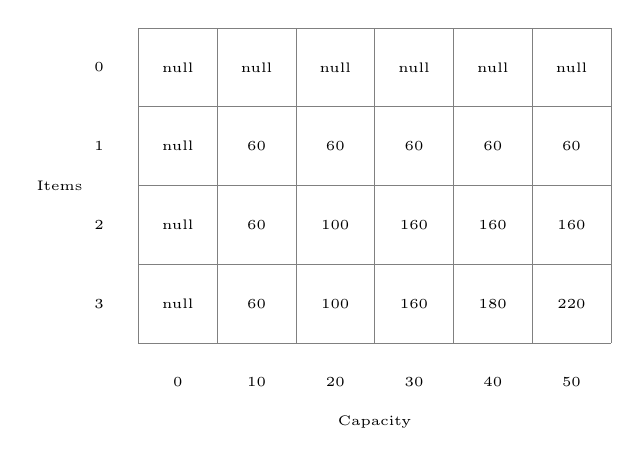
\begin{tikzpicture}
\draw[step=1cm,gray,very thin] (0,0) grid (6,4);
\node at (0.5,3.5) {\tiny null};
\node at (1.5,3.5) {\tiny null};
\node at (2.5,3.5) {\tiny null};
\node at (3.5,3.5) {\tiny null};
\node at (4.5,3.5) {\tiny null};
\node at (5.5,3.5) {\tiny null};

\node at (0.5,2.5) {\tiny null};
\node at (1.5,2.5) {\tiny 60};
\node at (2.5,2.5) {\tiny 60};
\node at (3.5,2.5) {\tiny 60};
\node at (4.5,2.5) {\tiny 60};
\node at (5.5,2.5) {\tiny 60};

\node at (0.5,1.5) {\tiny null};
\node at (1.5,1.5) {\tiny 60};
\node at (2.5,1.5) {\tiny 100};
\node at (3.5,1.5) {\tiny 160};
\node at (4.5,1.5) {\tiny 160};
\node at (5.5,1.5) {\tiny 160};

\node at (0.5,0.5) {\tiny null};
\node at (1.5,0.5) {\tiny 60};
\node at (2.5,0.5) {\tiny 100};
\node at (3.5,0.5) {\tiny 160};
\node at (4.5,0.5) {\tiny 180};
\node at (5.5,0.5) {\tiny 220};

% Labels
\node at (-0.5,3.5) {\tiny 0};
\node at (-0.5,2.5) {\tiny 1};
\node at (-0.5,1.5) {\tiny 2};
\node at (-0.5,0.5) {\tiny 3};

\node at (0.5,-0.5) {\tiny 0};
\node at (1.5,-0.5) {\tiny 10};
\node at (2.5,-0.5) {\tiny 20};
\node at (3.5,-0.5) {\tiny 30};
\node at (4.5,-0.5) {\tiny 40};
\node at (5.5,-0.5) {\tiny 50};

\node at (-1,2) {\tiny Items};
\node at (3,-1) {\tiny Capacity};
\end{tikzpicture}
\caption{Memoization table being filled during computation}
\end{figure}

\subsubsection{Algorithm}
\begin{algorithm}
\caption{0-1 Knapsack - Memoization}
\begin{algorithmic}
\REQUIRE Arrays $weights[]$, $values[]$, capacity $W$, number of items $n$, memo table $memo[][]$
\ENSURE Maximum value that can be obtained
\STATE \textbf{function} knapsackMemo($weights$, $values$, $W$, $n$, $memo$)
\IF{$n = 0$ OR $W = 0$}
    \RETURN 0
\ENDIF
\IF{$memo[n][W] \neq null$}
    \RETURN $memo[n][W]$
\ENDIF
\IF{$weights[n-1] \leq W$}
    \STATE $include = values[n-1] + $ knapsackMemo($weights$, $values$, $W - weights[n-1]$, $n-1$, $memo$)
    \STATE $exclude = $ knapsackMemo($weights$, $values$, $W$, $n-1$, $memo$)
    \STATE $memo[n][W] = \max(include, exclude)$
\ELSE
    \STATE $memo[n][W] = $ knapsackMemo($weights$, $values$, $W$, $n-1$, $memo$)
\ENDIF
\RETURN $memo[n][W]$
\end{algorithmic}
\end{algorithm}

\subsubsection{Java Implementation}
\begin{lstlisting}[caption=Memoization Solution]
static int KnapsackMemoization(int[] weights, int[] values, int capacity, 
                              int n, Integer[][] d) {
    // Base case: no items left or capacity is 0
    if (n == 0 || capacity == 0) {
        return 0;
    }
    
    // If the value is already computed, return it
    if (d[n][capacity] != null) {
        return d[n][capacity];
    }
    
    // If the weight of the nth item is less than or equal to the capacity
    if (weights[n - 1] <= capacity) {
        // Include the nth item and check the value with and without it
        int includeItem = values[n - 1] + KnapsackMemoization(weights, values, 
                         capacity - weights[n - 1], n - 1, d);
        int excludeItem = KnapsackMemoization(weights, values, capacity, n - 1, d);
        d[n][capacity] = Math.max(includeItem, excludeItem);
    } else {
        // If the nth item cannot be included, skip it
        d[n][capacity] = KnapsackMemoization(weights, values, capacity, n - 1, d);
    }
    return d[n][capacity]; 
}
\end{lstlisting}

\subsubsection{Complexity Analysis}
\textbf{Time Complexity:} $O(n \times W)$ - Each subproblem solved exactly once

\textbf{Space Complexity:} $O(n \times W)$ - Memoization table + $O(n)$ recursion stack

\subsection{Approach 3: Tabulation (Bottom-Up DP)}

\subsubsection{Key Insight}
Instead of recursion, we build the solution iteratively from the ground up. We systematically fill a 2D table where each cell represents the optimal solution for a subproblem.

\subsubsection{Table Interpretation}
$dp[i][w]$ = "Maximum value achievable using the first $i$ items with knapsack capacity $w$"

\subsubsection{Recurrence Relation}
\begin{equation}
dp[i][w] = \begin{cases}
0 & \text{if } i = 0 \text{ or } w = 0 \\
dp[i-1][w] & \text{if } weights[i-1] > w \\
\max(dp[i-1][w], dp[i-1][w-weights[i-1]] + values[i-1]) & \text{otherwise}
\end{cases}
\end{equation}

\subsubsection{Step-by-Step Table Construction}

\textbf{Step 1: Initialize base cases}
\begin{center}
\begin{tabular}{|c|c|c|c|c|c|c|}
\hline
\textbf{i\textbackslash w} & \textbf{0} & \textbf{10} & \textbf{20} & \textbf{30} & \textbf{40} & \textbf{50} \\
\hline
\textbf{0} & 0 & 0 & 0 & 0 & 0 & 0 \\
\hline
\textbf{1} & 0 & ? & ? & ? & ? & ? \\
\hline
\textbf{2} & 0 & ? & ? & ? & ? & ? \\
\hline
\textbf{3} & 0 & ? & ? & ? & ? & ? \\
\hline
\end{tabular}
\end{center}

\textbf{Step 2: Fill row 1 (Item 1: weight=10, value=60)}
\begin{center}
\begin{tabular}{|c|c|c|c|c|c|c|}
\hline
\textbf{i\textbackslash w} & \textbf{0} & \textbf{10} & \textbf{20} & \textbf{30} & \textbf{40} & \textbf{50} \\
\hline
\textbf{0} & 0 & 0 & 0 & 0 & 0 & 0 \\
\hline
\textbf{1} & 0 & 60 & 60 & 60 & 60 & 60 \\
\hline
\textbf{2} & 0 & ? & ? & ? & ? & ? \\
\hline
\textbf{3} & 0 & ? & ? & ? & ? & ? \\
\hline
\end{tabular}
\end{center}

\textbf{Step 3: Fill row 2 (Item 2: weight=20, value=100)}
\begin{center}
\begin{tabular}{|c|c|c|c|c|c|c|}
\hline
\textbf{i\textbackslash w} & \textbf{0} & \textbf{10} & \textbf{20} & \textbf{30} & \textbf{40} & \textbf{50} \\
\hline
\textbf{0} & 0 & 0 & 0 & 0 & 0 & 0 \\
\hline
\textbf{1} & 0 & 60 & 60 & 60 & 60 & 60 \\
\hline
\textbf{2} & 0 & 60 & 100 & 160 & 160 & 160 \\
\hline
\textbf{3} & 0 & ? & ? & ? & ? & ? \\
\hline
\end{tabular}
\end{center}

\textbf{Step 4: Fill row 3 (Item 3: weight=30, value=120)}
\begin{center}
\begin{tabular}{|c|c|c|c|c|c|c|}
\hline
\textbf{i\textbackslash w} & \textbf{0} & \textbf{10} & \textbf{20} & \textbf{30} & \textbf{40} & \textbf{50} \\
\hline
\textbf{0} & 0 & 0 & 0 & 0 & 0 & 0 \\
\hline
\textbf{1} & 0 & 60 & 60 & 60 & 60 & 60 \\
\hline
\textbf{2} & 0 & 60 & 100 & 160 & 160 & 160 \\
\hline
\textbf{3} & 0 & 60 & 100 & 160 & 180 & \textbf{220} \\
\hline
\end{tabular}
\end{center}

\subsubsection{Algorithm}
\begin{algorithm}
\caption{0-1 Knapsack - Tabulation}
\begin{algorithmic}
\REQUIRE Arrays $weights[]$, $values[]$, capacity $W$
\ENSURE Maximum value that can be obtained
\STATE $n \leftarrow$ length of $weights[]$
\STATE Create 2D array $dp[n+1][W+1]$ initialized to 0
\FOR{$i = 1$ to $n$}
    \FOR{$w = 0$ to $W$}
        \IF{$weights[i-1] \leq w$}
            \STATE $dp[i][w] \leftarrow \max(dp[i-1][w], dp[i-1][w-weights[i-1]] + values[i-1])$
        \ELSE
            \STATE $dp[i][w] \leftarrow dp[i-1][w]$
        \ENDIF
    \ENDFOR
\ENDFOR
\RETURN $dp[n][W]$
\end{algorithmic}
\end{algorithm}

\subsubsection{Java Implementation}
\begin{lstlisting}[caption=Tabulation Solution]
static int KnapsackTabulation(int[] weights, int[] values, int capacity) {
    int n = weights.length;
    int[][] dp = new int[n + 1][capacity + 1];

    // dp[i][w] will store the maximum value that can be obtained 
    // with the first i items and capacity w

    // Build the dp table in bottom-up manner
    for (int i = 1; i <= n; i++) {
        for (int w = 0; w <= capacity; w++) {
            if (weights[i - 1] <= w) {
                dp[i][w] = Math.max(dp[i - 1][w], 
                          dp[i - 1][w - weights[i - 1]] + values[i - 1]); 
            } else {
                dp[i][w] = dp[i - 1][w];
            }
        }
    }
    return dp[n][capacity];
}
\end{lstlisting}

\subsubsection{Complexity Analysis}
\textbf{Time Complexity:} $O(n \times W)$ - Two nested loops

\textbf{Space Complexity:} $O(n \times W)$ - 2D DP table

\section{Detailed Example Walkthrough}

Let's trace through our hiking example step by step using tabulation:

\textbf{Given:}
\begin{itemize}
\item Items: Tent (10 lbs, \$60), Sleeping Bag (20 lbs, \$100), Food (30 lbs, \$120)
\item Capacity: 50 lbs
\end{itemize}

\subsection{Filling dp[1][w] (First item: Tent)}
For each capacity $w$ from 0 to 50:
\begin{itemize}
\item $w < 10$: Cannot include tent, so $dp[1][w] = dp[0][w] = 0$
\item $w \geq 10$: Can include tent
    \begin{itemize}
    \item Include: $dp[0][w-10] + 60 = 0 + 60 = 60$
    \item Exclude: $dp[0][w] = 0$
    \item Choose max: $dp[1][w] = 60$
    \end{itemize}
\end{itemize}

\subsection{Filling dp[2][30] (Adding sleeping bag, capacity 30)}
\begin{itemize}
\item Can we include sleeping bag (weight 20)? Yes, $20 \leq 30$
\item Include sleeping bag: $dp[1][30-20] + 100 = dp[1][10] + 100 = 60 + 100 = 160$
\item Exclude sleeping bag: $dp[1][30] = 60$
\item Choose max: $dp[2][30] = \max(160, 60) = 160$
\end{itemize}

\subsection{Filling dp[3][50] (Adding food, capacity 50)}
\begin{itemize}
\item Can we include food (weight 30)? Yes, $30 \leq 50$
\item Include food: $dp[2][50-30] + 120 = dp[2][20] + 120 = 100 + 120 = 220$
\item Exclude food: $dp[2][50] = 160$
\item Choose max: $dp[3][50] = \max(220, 160) = 220$
\end{itemize}

\textbf{Note:} The value $220 represents Sleeping Bag + Food (20+30=50 lbs, exactly at capacity).
This is the globally optimal solution. Tent + Food (10+30=40 lbs, $180) is another valid combination that uses less capacity.

\textbf{Final Answer:} The maximum value is \$220 (Sleeping Bag + Food combination).

\section{Finding the Actual Items Selected}

To find which items were selected, we trace back through the DP table:

\begin{algorithm}
\caption{Backtracking to Find Selected Items}
\begin{algorithmic}
\STATE $i \leftarrow n$, $w \leftarrow W$
\STATE Create empty list $selectedItems$
\WHILE{$i > 0$ AND $w > 0$}
    \IF{$dp[i][w] \neq dp[i-1][w]$}
        \STATE Add item $i$ to $selectedItems$
        \STATE $w \leftarrow w - weights[i-1]$
    \ENDIF
    \STATE $i \leftarrow i - 1$
\ENDWHILE
\RETURN $selectedItems$
\end{algorithmic}
\end{algorithm}

\section{Space Optimization}

Since each row only depends on the previous row, we can optimize space to $O(W)$:

\begin{lstlisting}[caption=Space-Optimized Tabulation]
static int KnapsackOptimized(int[] weights, int[] values, int capacity) {
    int n = weights.length;
    int[] dp = new int[capacity + 1];
    
    for (int i = 0; i < n; i++) {
        // Traverse from right to left to avoid using updated values
        for (int w = capacity; w >= weights[i]; w--) {
            dp[w] = Math.max(dp[w], dp[w - weights[i]] + values[i]);
        }
    }
    return dp[capacity];
}
\end{lstlisting}

\textbf{Key Insight:} We traverse from right to left to ensure we don't use already updated values from the current iteration.

\section{Comparison of Approaches}

\begin{table}[h]
\centering
\begin{tabular}{|l|c|c|c|c|}
\hline
\textbf{Approach} & \textbf{Time} & \textbf{Space} & \textbf{Practical Limit} & \textbf{Pros/Cons} \\
\hline
Naive Recursion & $O(2^n)$ & $O(n)$ & $n \leq 20$ & Simple but inefficient \\
\hline
Memoization & $O(n \times W)$ & $O(n \times W)$ & $n, W \leq 1000$ & Top-down, intuitive \\
\hline
Tabulation & $O(n \times W)$ & $O(n \times W)$ & $n, W \leq 1000$ & Bottom-up, iterative \\
\hline
Space Optimized & $O(n \times W)$ & $O(W)$ & $W \leq 10^6$ & Memory efficient \\
\hline
\end{tabular}
\caption{Comparison of different approaches}
\end{table}

\section{Variations and Extensions}

\subsection{Fractional Knapsack}
Unlike 0-1 Knapsack, items can be broken into fractions. This can be solved greedily by value-to-weight ratio.

\subsection{Unbounded Knapsack}
Each item can be used multiple times. The recurrence becomes:
$$dp[i][w] = \max(dp[i-1][w], dp[i][w-weights[i-1]] + values[i-1])$$

\subsection{Multiple Knapsacks}
Multiple knapsacks with different capacities - requires 3D DP.

\subsection{Bounded Knapsack}
Each item has a limited quantity available.

\section{Real-World Applications}

\begin{enumerate}
\item \textbf{Resource Allocation:} Budget allocation across projects
\item \textbf{Portfolio Selection:} Investment selection with budget constraints
\item \textbf{Cargo Loading:} Optimizing cargo in ships/planes
\item \textbf{Memory Management:} Selecting data structures for limited memory
\item \textbf{Feature Selection:} Machine learning model optimization
\item \textbf{Network Optimization:} Bandwidth allocation
\end{enumerate}

\section{Common Pitfalls and Debugging Tips}

\subsection{Array Indexing}
\begin{itemize}
\item Remember: $weights[i-1]$ and $values[i-1]$ when $i$ represents the item number
\item DP table indices: $dp[i][w]$ where $i$ goes from 0 to $n$ and $w$ from 0 to $W$
\end{itemize}

\subsection{Base Cases}
\begin{itemize}
\item $dp[0][w] = 0$ for all $w$ (no items = no value)
\item $dp[i][0] = 0$ for all $i$ (no capacity = no value)
\end{itemize}

\subsection{Integer Overflow}
For large values, use \texttt{long} instead of \texttt{int}.

\subsection{Testing Strategy}
\begin{enumerate}
\item Test with simple cases (single item, zero capacity)
\item Verify against brute force for small inputs
\item Check edge cases (all items too heavy, all items fit)
\end{enumerate}

\section{Advanced Topics}

\subsection{Branch and Bound}
For exact solutions with better average-case performance than DP.

\subsection{Approximation Algorithms}
When exact solutions are too expensive:
\begin{itemize}
\item Greedy by value-to-weight ratio
\item FPTAS (Fully Polynomial-Time Approximation Scheme)
\end{itemize}

\subsection{Parallel Implementation}
DP table can be filled diagonally for parallel processing.

\section{Conclusion}

The 0-1 Knapsack problem is a cornerstone of dynamic programming, demonstrating:

\begin{itemize}
\item \textbf{Optimal Substructure:} Optimal solution contains optimal solutions to subproblems
\item \textbf{Overlapping Subproblems:} Same subproblems appear in different branches
\item \textbf{Trade-offs:} Time vs. space complexity considerations
\item \textbf{Problem Transformation:} Converting recursive solutions to iterative DP
\end{itemize}

\textbf{Key Takeaways:}
\begin{itemize}
\item Always start with recursive solution to understand the problem structure
\item Identify overlapping subproblems for memoization opportunities
\item Consider space optimization when memory is a constraint
\item Understand the problem constraints to choose the right approach
\end{itemize}

\textbf{Learning Objectives Achieved:}
\begin{itemize}
\item Understanding classical optimization problems
\item Implementing three DP paradigms (recursion, memoization, tabulation)
\item Analyzing time and space complexity trade-offs
\item Recognizing real-world applications of algorithmic concepts
\item Developing debugging and testing strategies for DP problems
\end{itemize}

\section{References}

\begin{enumerate}
\item Cormen, T. H., Leiserson, C. E., Rivest, R. L., \& Stein, C. (2009). \textit{Introduction to Algorithms} (3rd ed.). MIT Press.
\item Kleinberg, J., \& Tardos, E. (2005). \textit{Algorithm Design}. Addison-Wesley.
\item Sedgewick, R., \& Wayne, K. (2011). \textit{Algorithms} (4th ed.). Addison-Wesley.
\item Dasgupta, S., Papadimitriou, C., \& Vazirani, U. (2006). \textit{Algorithms}. McGraw-Hill.
\item Dynamic Programming Problems and Applications in Computer Science
\end{enumerate}

\end{document}
